\documentclass[tikz,border=10pt]{standalone}
\usepackage{helvet}
\renewcommand{\familydefault}{\sfdefault}
\usepackage{tikz}
\usetikzlibrary{positioning, fit, calc, backgrounds}

\definecolor{emeraldpine}{HTML}{1A4D3E}
\definecolor{ethpetrol}{HTML}{007A87}
\definecolor{ethbronze}{HTML}{B87333}
\definecolor{ink}{HTML}{1A202C}
\definecolor{softink}{HTML}{4A5568}
\definecolor{brainbg}{HTML}{F7EDE3}
\definecolor{sysbg}{HTML}{E8F0EC}
\definecolor{worldbg}{HTML}{E3F3F5}

\begin{document}
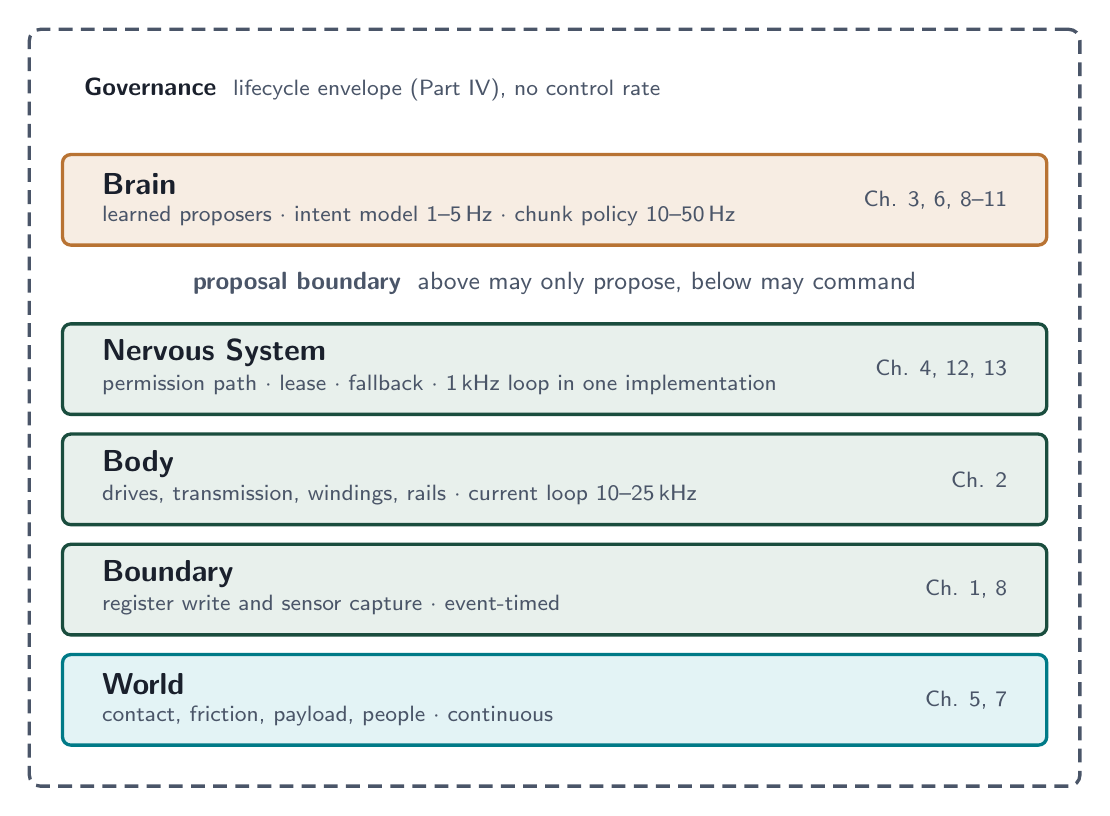
\begin{tikzpicture}[
    box/.style={
        rectangle, 
        rounded corners=3pt,
        minimum width=12.5cm,
        minimum height=1.15cm,
        inner sep=0pt,
        anchor=north,
        align=left
    },
    title/.style={
        font=\fontsize{10.5}{12}\selectfont\bfseries,
        text=ink,
        anchor=west
    },
    subtitle/.style={
        font=\fontsize{8.5}{10}\selectfont,
        text=softink,
        anchor=west
    },
    chap/.style={
        font=\fontsize{8.5}{10}\selectfont,
        text=softink,
        anchor=east
    }
]

% Governance Title
\node[anchor=west, font=\fontsize{9.5}{11}\selectfont\bfseries, text=ink] (gov_title) at (-6.1, 0.8) {Governance\hspace{6pt}\normalfont\fontsize{8.5}{10}\selectfont\color{softink}lifecycle envelope (Part IV), no control rate};

% Brain
\node[box, fill=brainbg, draw=ethbronze, line width=1.2pt] (brain) at (0, 0) {};
\node[title] at ($(brain.west) + (0.4, 0.2)$) {Brain};
\node[subtitle] at ($(brain.west) + (0.4, -0.2)$) {learned proposers $\cdot$ intent model 1--5\,Hz $\cdot$ chunk policy 10--50\,Hz};
\node[chap] at ($(brain.east) + (-0.4, 0)$) {Ch. 3, 6, 8--11};

% Proposal Boundary
\node[anchor=center, font=\fontsize{9}{11}\selectfont\itshape\bfseries, text=softink] (prop_bound) at (0, -1.65) {proposal boundary\hspace{6pt}\normalfont\fontsize{9}{11}\selectfont above may only propose, below may command};

% Nervous System
\node[box, fill=sysbg, draw=emeraldpine, line width=1.2pt] (nervous) at (0, -2.15) {};
\node[title] at ($(nervous.west) + (0.4, 0.2)$) {Nervous System};
\node[subtitle] at ($(nervous.west) + (0.4, -0.2)$) {permission path $\cdot$ lease $\cdot$ fallback $\cdot$ 1\,kHz loop in one implementation};
\node[chap] at ($(nervous.east) + (-0.4, 0)$) {Ch. 4, 12, 13};

% Body
\node[box, fill=sysbg, draw=emeraldpine, line width=1.2pt] (body) at (0, -3.55) {};
\node[title] at ($(body.west) + (0.4, 0.2)$) {Body};
\node[subtitle] at ($(body.west) + (0.4, -0.2)$) {drives, transmission, windings, rails $\cdot$ current loop 10--25\,kHz};
\node[chap] at ($(body.east) + (-0.4, 0)$) {Ch. 2};

% Boundary
\node[box, fill=sysbg, draw=emeraldpine, line width=1.2pt] (boundary) at (0, -4.95) {};
\node[title] at ($(boundary.west) + (0.4, 0.2)$) {Boundary};
\node[subtitle] at ($(boundary.west) + (0.4, -0.2)$) {register write and sensor capture $\cdot$ event-timed};
\node[chap] at ($(boundary.east) + (-0.4, 0)$) {Ch. 1, 8};

% World
\node[box, fill=worldbg, draw=ethpetrol, line width=1.2pt] (world) at (0, -6.35) {};
\node[title] at ($(world.west) + (0.4, 0.2)$) {World};
\node[subtitle] at ($(world.west) + (0.4, -0.2)$) {contact, friction, payload, people $\cdot$ continuous};
\node[chap] at ($(world.east) + (-0.4, 0)$) {Ch. 5, 7};

% Governance Background (drawn last but put in background layer)
\begin{scope}[on background layer]
\node[rectangle, rounded corners=4pt, draw=softink, line width=1.2pt, dashed, dash pattern=on 5pt off 3pt, 
      inner xsep=0.4cm, inner ysep=0.5cm, fit=(gov_title) (brain) (world)] (gov) {};
\end{scope}

\end{tikzpicture}
\end{document}
